%! TeX program = lualatex
\documentclass[12pt,a4paper]{article}

\usepackage[nil]{babel}
\usepackage{unicode-math}
\usepackage[svgnames]{xcolor}
\usepackage{lmodern}
\usepackage{graphicx}
\usepackage{wrapfig}
\usepackage{float}
\usepackage{parskip}

\babelprovide[import=el, main, onchar=ids fonts]{greek} % can also do import=el-polyton
\babelprovide[import, onchar=ids fonts]{english}

\babelfont{rm}
          [Language=Default]{Liberation Sans}
\babelfont[english]{rm}
          [Language=Default]{Liberation Sans}
\babelfont{sf}
          [Language=Default]{Liberation Sans}
\babelfont{tt}
          [Language=Default]{Liberation Sans}

%Enter Title Here
 \title{Robustness-diagrams-v0.1 \\ LibShare}
\author{\textbf{Ονόματα / ΑΜ / Έτος:} \\ Γρηγόρης Καπαδούκας / 1072484 / 4\textdegree \\ Χρήστος Μπεστητζάνος / 1072615 / 4\textdegree \\ Νικόλαος Αυγέρης / 1067508 / 5\textdegree \\ Περικλής Κοροντζής / 1072563 / 4\textdegree}

\begin{document}

\makeatletter
\begin{center}
	\LARGE{\@title} \\
	\pagebreak
    \begin{LARGE}\@author\end{LARGE}
    \pagebreak
\end{center}

%Insert Body Here
\section{Robustness Diagrams}

\subsection{Αναζήτηση βιβλίων / χρήστη / αιτήσεων}
\begin{figure}[H]
	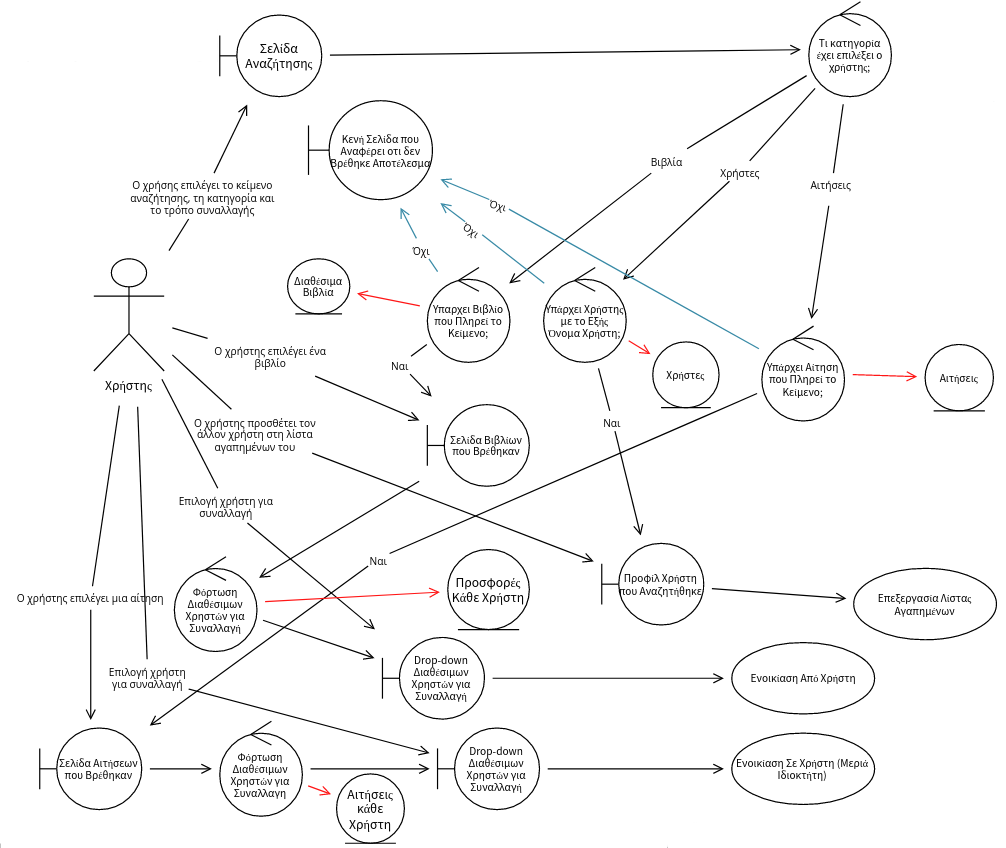
\includegraphics[width=\textwidth]{Search Robustness.png}
	\caption{Robustness Diagram: Αναζήτηση βιβλίων / χρήστη / αιτήσεων}
	\label{Robustness Diagram: Αναζήτηση βιβλίων / χρήστη / αιτήσεων}
\end{figure}

\subsection{Ενοικίαση βιβλίου από άλλο χρήστη}
\begin{figure}[H]
	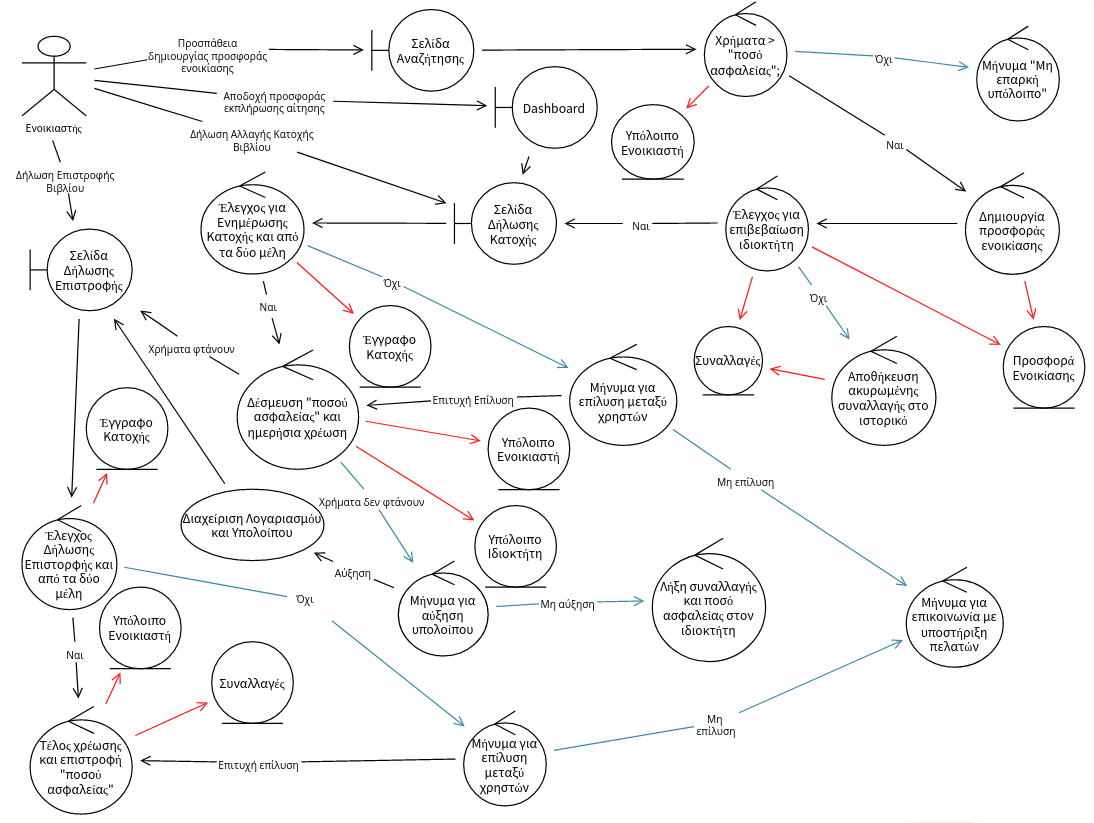
\includegraphics[width=\textwidth]{Rent from User Robustness.png}
	\caption{Robustness Diagram: Ενοικίαση βιβλίου από άλλο χρήστη}
	\label{Robustness Diagram: Ενοικίαση βιβλίου από άλλο χρήστη}
\end{figure}

\subsection{Ενοικίαση βιβλίου σε άλλο χρήστη (μεριά ιδιοκτήτη)}
\begin{figure}[H]
	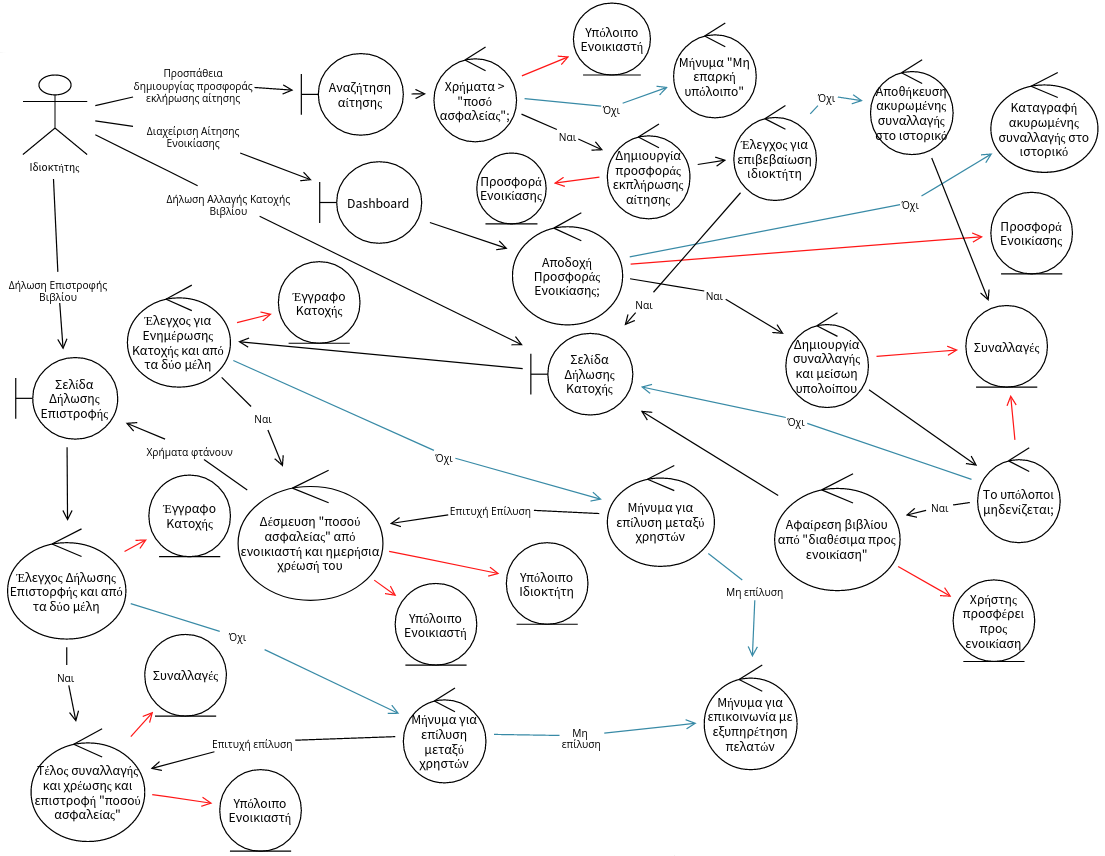
\includegraphics[width=\textwidth]{Rent to User Robustness.png}
	\caption{Robustness Diagram: Ενοικίαση βιβλίου σε άλλο χρήστη (μεριά ιδιοκτήτη)}
	\label{Robustness Diagram: Ενοικίαση βιβλίου σε άλλο χρήστη μεριά ιδιοκτήτη}
\end{figure}

\subsection{Διαχείριση των βιβλίων που προσφέρει ο χρήστης προς ενοικίαση από άλλους}
\begin{figure}[H]
	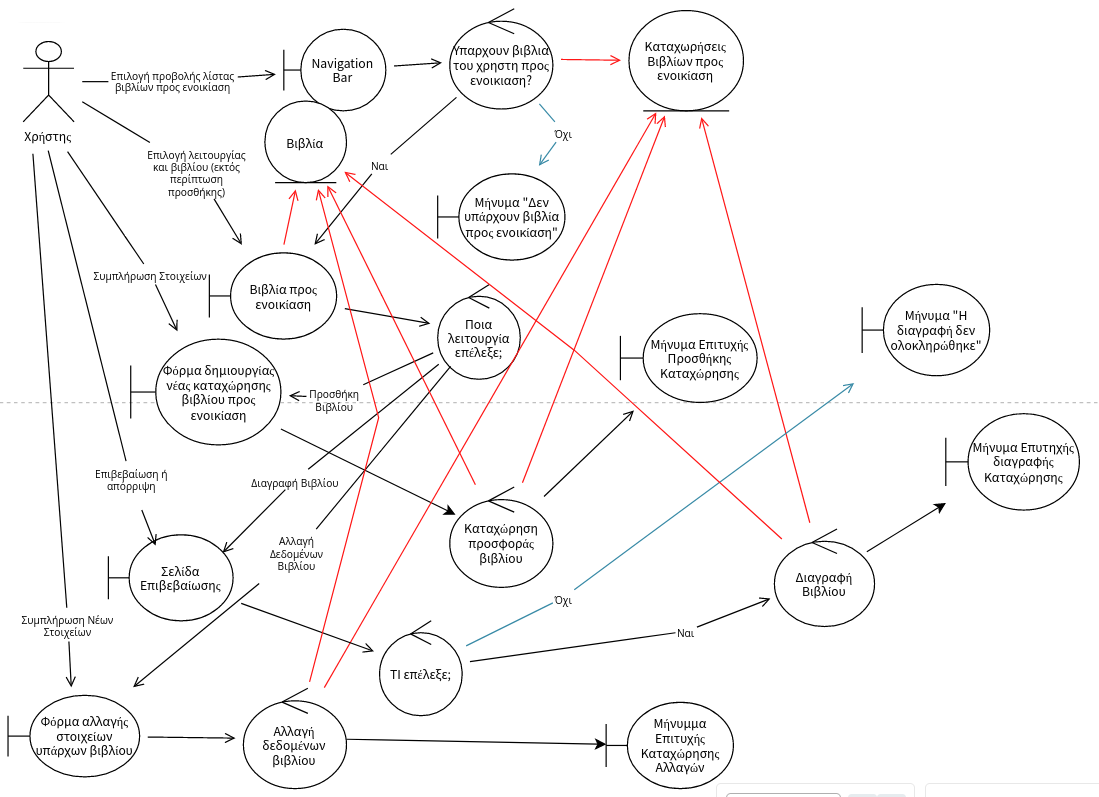
\includegraphics[width=\textwidth]{Manage User Book Listings Robustness.png}
	\caption{Robustness Diagram: Διαχείριση των βιβλίων που προσφέρει ο χρήστης προς ενοικίαση από άλλους}
	\label{Robustness Diagram: Διαχείριση των βιβλίων που προσφέρει ο χρήστης προς ενοικίαση από άλλους}
\end{figure}

\subsection{Διαχείριση των αιτήσεων που έχει κάνει ο χρήστης}
\begin{figure}[H]
	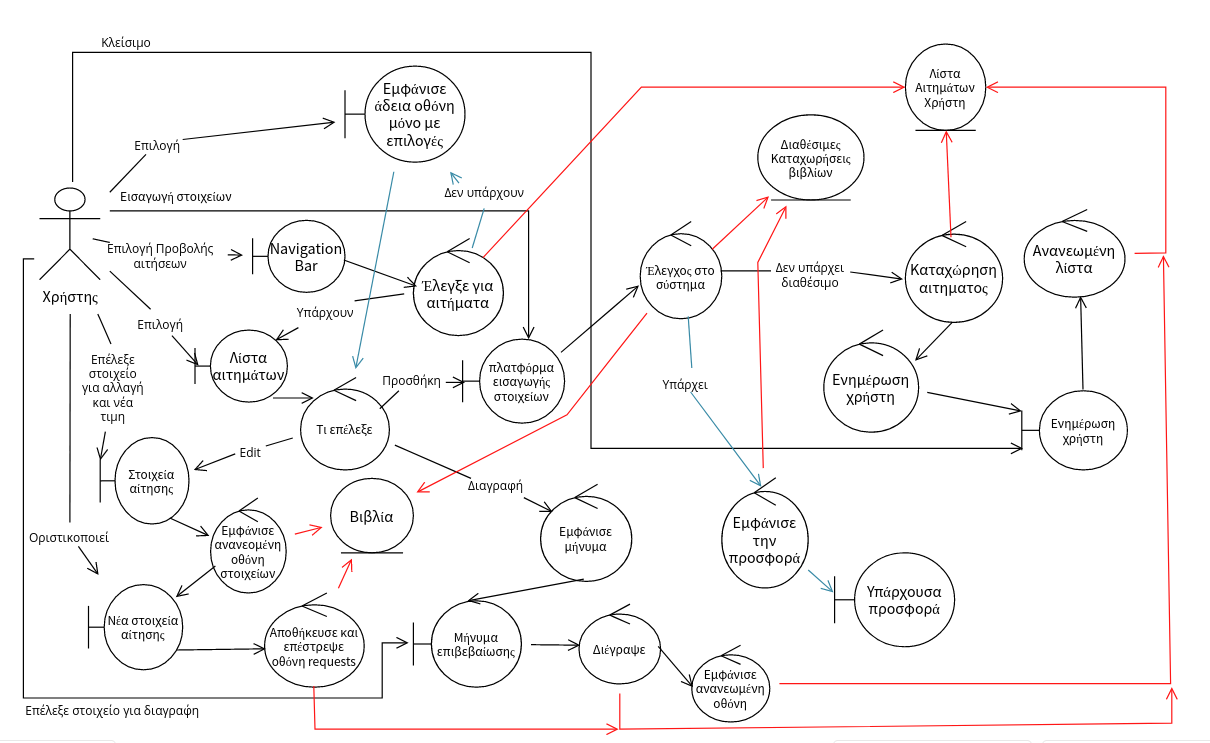
\includegraphics[width=\textwidth]{Manage User Requests Robustness.png}
	\caption{Robustness Diagram: Διαχείριση των αιτήσεων που έχει κάνει ο χρήστης}
	\label{Robustness Diagram: Διαχείριση των αιτήσεων που έχει κάνει ο χρήστης}
\end{figure}

\subsection{Αξιολόγηση άλλων χρηστών μετά από την ολοκλήρωση συναλλαγής}
\begin{figure}[H]
	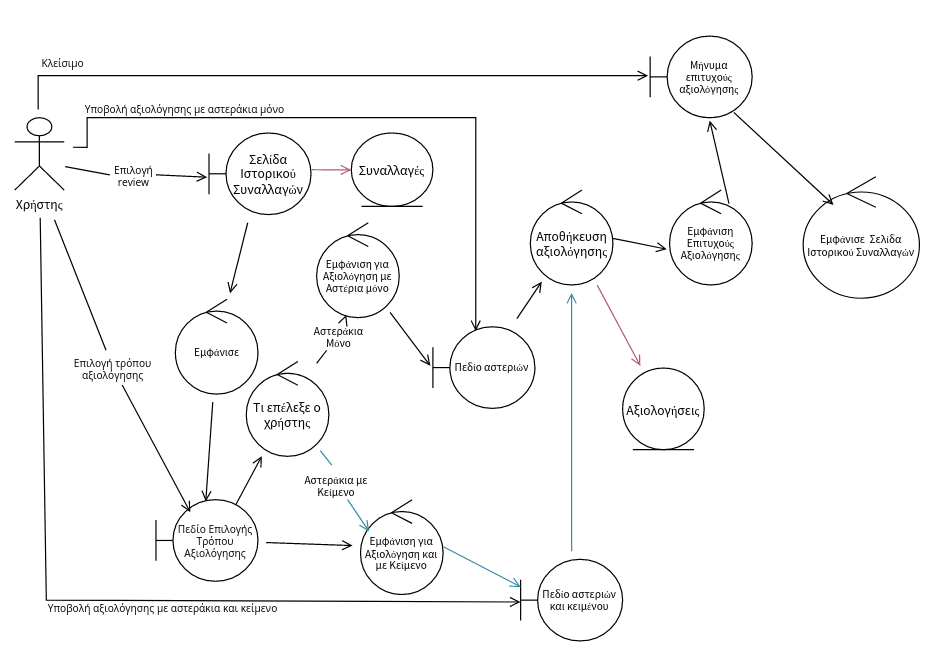
\includegraphics[width=\textwidth]{Review after Transaction Robustness.png}
	\caption{Robustness Diagram: Αξιολόγηση άλλων χρηστών μετά από την ολοκλήρωση συναλλαγής}
	\label{Robustness Diagram: Αξιολόγηση άλλων χρηστών μετά από την ολοκλήρωση συναλλαγής}
\end{figure}


\subsection{Προβολή και Επεξεργασία στοιχείων λογαριασμού χρήστη}
\begin{figure}[H]
	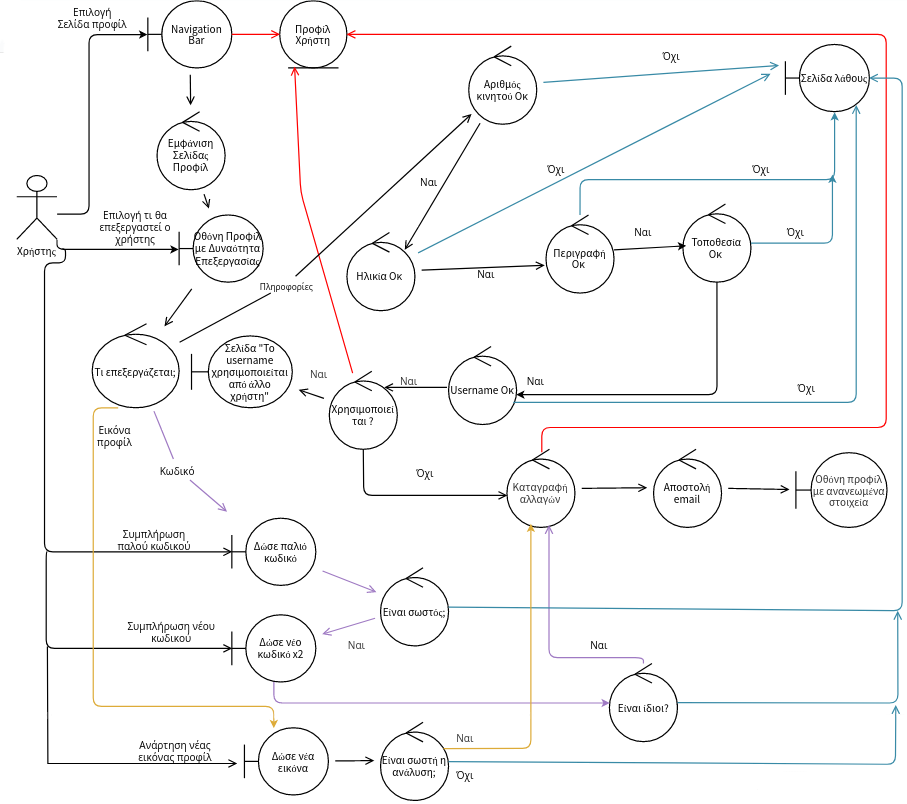
\includegraphics[width=\textwidth]{View and Edit User Account Details Robustness.png}
	\caption{Robustness Diagram: Προβολή και Επεξεργασία στοιχείων λογαριασμού χρήστη}
	\label{Robustness Diagram: Προβολή και Επεξεργασία στοιχείων λογαριασμού χρήστη}
\end{figure}

\subsection{Επεξεργασία χρηματικού υπολοίπου χρήστη}
\begin{figure}[H]
	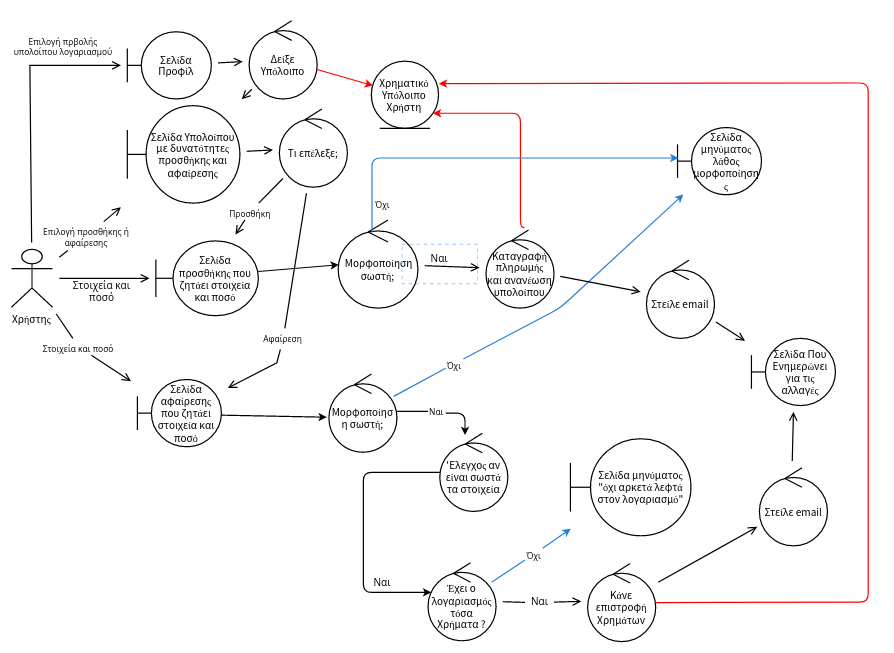
\includegraphics[width=\textwidth]{Edit User Balance Robustness.png}
	\caption{Robustness Diagram: Επεξεργασία χρηματικού υπολοίπου χρήστη}
	\label{Robustness Diagram: Επεξεργασία χρηματικού υπολοίπου χρήστη}
\end{figure}

\subsection{Επεξεργασία λίστας αγαπημένων και χρήση συστήματος ειδοποιήσεων}
\begin{figure}[H]
	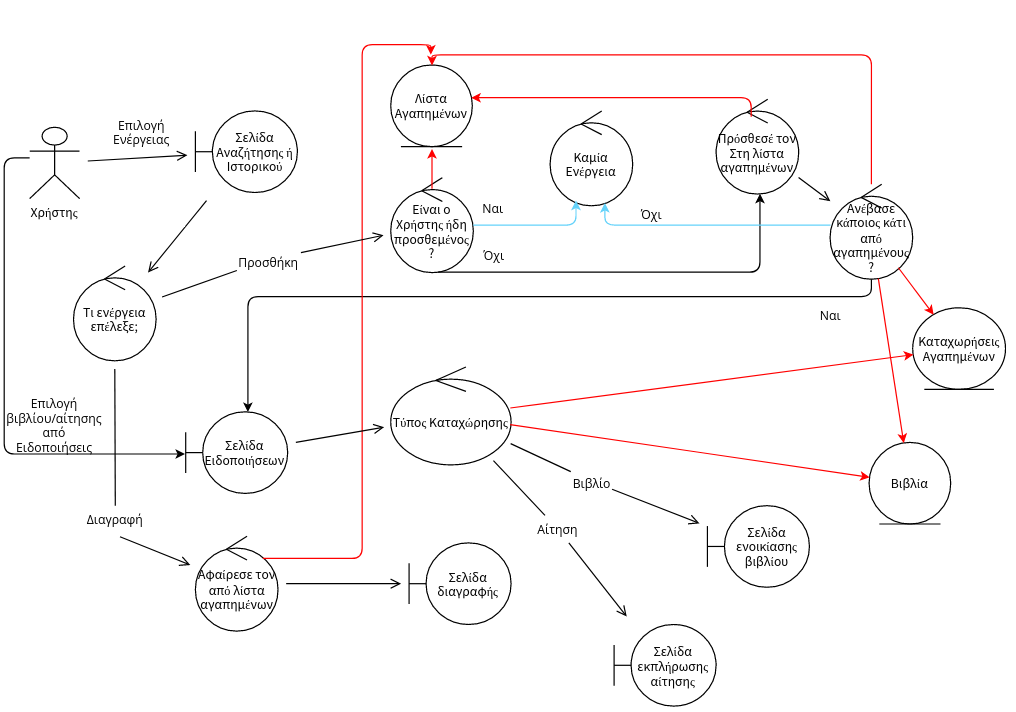
\includegraphics[width=\textwidth]{Favorite Users and Notification System Robustness.png}
	\caption{Robustness Diagram: Επεξεργασία λίστας αγαπημένων και χρήση συστήματος ειδοποιήσεων}
	\label{Robustness Diagram: Επεξεργασία λίστας αγαπημένων και χρήση συστήματος ειδοποιήσεων}
\end{figure}

\subsection{Προβολή ιστορικού συναλλαγών και στατιστικών}
\begin{figure}[H]
	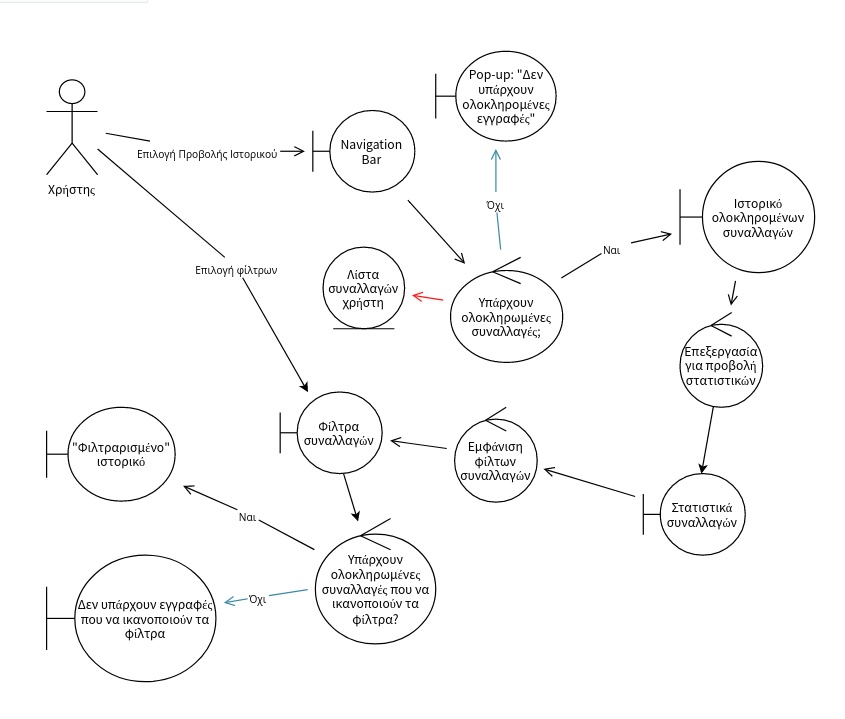
\includegraphics[width=\textwidth]{History and Statistics Robustness.png}
	\caption{Robustness Diagram: Προβολή ιστορικού συναλλαγών και στατιστικών}
	\label{Robustness Diagram: Προβολή ιστορικού συναλλαγών και στατιστικών}
\end{figure}

\section{Συμμετοχή και Ρόλοι στη Συγγραφή του Κειμένου}
\begin{enumerate}
	\item \textbf{Γρηγόρης Καπαδούκας:} Author (Κεφαλαίων 1, 2.1, 2.2, 2.3), Editor Όλων, Reviewer Όλων
	\item \textbf{Χρήστος Μπεστητζάνος:} Author (Κεφαλαίων 2.5, 2.6)
   	\item \textbf{Νικόλαος Αυγέρης:} Author (Κεφαλαίων 2.7, 2.8, 2.9)
	\item \textbf{Περικλής Κοροντζής:} Author (Κεφαλαίων 2.4, 2.10)
\end{enumerate}

\end{document}
